\documentclass[../notes.tex]{subfiles}

\pagestyle{main}
\renewcommand{\chaptermark}[1]{\markboth{\chaptername\ \thechapter\ (#1)}{}}
\setcounter{chapter}{3}

\begin{document}




\chapter{Entropy and the Second Law of Thermodynamics}
\section{Entropy Equations}
\begin{itemize}
    \item \marginnote{1/31:}We define a new state function $S$ by $\dd{S}=\var{q_\text{rev}}/T$ and call it \textbf{entropy}.
    \begin{itemize}
        \item See notes from last time for why this is a state function.
    \end{itemize}
    \item Verify that the same definition of entropy is a state function for any system.
    \begin{itemize}
        \item Consider an ideal gas system in thermal equilibrium with an arbitrary system and drive the ideal gas system along a loop.
        \item Around the cycle: $\Delta S_\text{total}=0$.
        \item Ideal gas:
        \begin{align*}
            \Delta S_\text{total} &= \Delta S_1+\Delta S_2\\
            &= \int\frac{\var{q_{\text{rev}_1}}}{T}-\int\frac{\var{q_{\text{rev}_1}}}{T}\\
            &= \int\frac{\var{q_{\text{rev}_1}}}{T}+\int\frac{\var{q_{\text{rev}_2}}}{T}
        \end{align*}
    \end{itemize}
    \item We must devise a reversible process to calculate the entropy changes for an irreversible process leading to the same final state.
    \begin{figure}[h!]
        \centering
        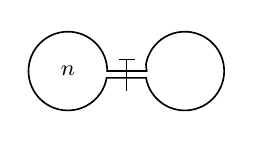
\begin{tikzpicture}
            \footnotesize
            \draw [semithick] (0.5,0) -- (0,0) arc[start angle=0,end angle=350,radius=5mm] -- ++(0.5,0) arc[start angle=-170,end angle=170,radius=5mm] -- cycle;
    
            \draw (0.25,-0.25) -- ++(0,0.4) ++(-0.1,0) -- ++(0.2,0);
    
            \node [left=3mm] {$n$};
        \end{tikzpicture}
        \caption{Two linked containers.}
        \label{fig:linkedContainers}
    \end{figure}
    \begin{itemize}
        \item Imagine two linked containers, one filled with $n$ moles of gas and the other vacuumed.
        \item Opening the two containers to each other results in an adiabatic expansion. All vibrational/rotational energy of the molecules is consumed and used for translation.
        \item Measuring the temperature with spectroscopy (the Maxwell-Boltzmann distribution of each spectral line, plus only the ground rovibrational states are occupied now) shows a drastic drop in temperature.
        \item We have $\var{q}=0$ and $\var{w}=0$ so that $\dd{U}=0$ and $\Delta T=0$ overall?
        \item An isothermal expansion is a reversible process leading to the same final state.
        \item $\dd{U}=0$ implies $\var{q_\text{rev}}=-\var{w}=P\dd{V}$.
        \item We have that
        \begin{equation*}
            \Delta S = \int\frac{\var{q_\text{rev}}}{T}
            = \int_{V_0}^{2V_0}\frac{P\dd{V}}{T}
            = \int_{V_0}^{2V_0}\frac{nRT}{V}\frac{1}{T}\dd{V}
            = nR\ln 2
        \end{equation*}
    \end{itemize}
    \item Using entropy as a state function to predict the vapor pressure in equilibrium with its liquid, from the enthalpy at boiling and the boiling temperature.
    \begin{figure}[h!]
        \centering
        \begin{tikzpicture}
            \footnotesize
            \node (a) at (0,0)  {\ce{H2O_{(l)}} $T  ,P_0$};
            \node (b) at (0,-2) {\ce{H2O_{(l)}} $T_b,P_0$};
            \node (c) at (4,-2) {\ce{H2O_{(g)}} $T_b,P_0$};
            \node (d) at (4,-1) {\ce{H2O_{(g)}} $T_b,P  $};
            \node (e) at (4,0)  {\ce{H2O_{(g)}} $T  ,P  $};
    
            \draw [-stealth,semithick] (a) -- node[above]{$\Delta S_0$} (e);
            \draw [-stealth,semithick] (a) -- node[left ]{$\Delta S_1$} (b);
            \draw [-stealth,semithick] (b) -- node[below]{$\Delta S_2$} (c);
            \draw [-stealth,semithick] (c) -- node[right]{$\Delta S_3$} (d);
            \draw [-stealth,semithick] (d) -- node[right]{$\Delta S_4$} (e);
        \end{tikzpicture}
        \caption{Vapor pressure thermodynamic loop.}
        \label{fig:thermodynamicLoop}
    \end{figure}
    \begin{itemize}
        \item Consider the above thermodynamic loop, where $T$ is the temperature of the water and $P$ is the pressure above the water.
        \item We have that
        \begin{align*}
            \Delta S_1 &= \int_T^{T_b}\frac{C_{P_l}}{T}\dd{T}&
            \Delta S_2 &= \frac{\Delta H_\text{vap}}{T_b}&
            \Delta S_3 &= nR\ln\frac{P_0}{P}&
            \Delta S_4 &= \int_{T_b}^T\frac{C_{P_g}}{T}\dd{T}
        \end{align*}
        and that
        \begin{equation*}
            \Delta S_0 = \frac{\Delta H_\text{vap}}{T}
        \end{equation*}
        \item We know that $\Delta S$ around the loop is zero since $S$ is a state function. We neglect the heat capacity effect. Thus,
        \begin{align*}
            \frac{\Delta H_\text{vap}}{T_b}+nR\ln\frac{P_0}{P}-\frac{\Delta H_\text{vap}}{T} &= 0\\
            \ln\frac{P_0}{P} &= \frac{\Delta H_\text{vap}}{nR}\left( \frac{1}{T}-\frac{1}{T_b} \right)\\
            P &= P_0\e[-\Delta H_\text{vap}/nR(1/T-1/T_b)]
        \end{align*}
        \item The above equation gives the vapor pressure at $T$ in terms of the vapor pressure $P_0$ at $T_b$.
    \end{itemize}
    \item \textbf{Trouton's rule}: The statement that
    \begin{equation*}
        \frac{\Delta H_\text{vap}}{T_b} \approx 85\pm\SI{5}{\joule\per\mole\per\kelvin}
    \end{equation*}
    \begin{itemize}
        \item Discovered this rule as an undergrad after an afternoon's manipulation of data from a book of tables.
        \item This rule reflects the fact that
        \begin{equation*}
            \frac{\Delta H_\text{vap}}{T_b} = \Delta S_\text{vap}
        \end{equation*}
        and implies that $\Delta S_\text{vap}$ is approximately a constant.
    \end{itemize}
    \item Example of entropy change: The direction of heat flow between two systems (1 and 2) only in thermal contact.
    \begin{itemize}
        \item We have
        \begin{align*}
            \var{q_{\text{rev}_1}} &= \var{q_{\text{rev}_2}}\\
            C_{V_1}\dd{T_1} &= -C_{V_2}\dd{T_2}
        \end{align*}
        \item Thus,
        \begin{align*}
            \dd{S} &= \dd{S_1}+\dd{S_2}\\
            &= \frac{\var{q_{\text{rev}_1}}}{T_1}+\frac{\var{q_{\text{rev}_2}}}{T_2}\\
            &= \frac{C_V\dd{T_1}}{T_1}-\frac{C_V\dd{T_1}}{T_2}\\
            &= C_V\dd{T_1}\left( \frac{1}{T_1}-\frac{1}{T_2} \right)
        \end{align*}
        \item The conclusion is that if $\dd{T_1}>0$, then $\dd{S}>0$. This is the spontaneous direction, the direction that nature chooses, the one in which entropy increases.
        \item The maximum of $S$ is the equilibrium temperature between the two systems.
    \end{itemize}
    \item Entropy change of the isothermal mixing of two ideal gases at the same temperature.
    \begin{itemize}
        \item Consider the same two-container setup from Figure \ref{fig:linkedContainers}.
        \item We have that
        \begin{align*}
            \Delta S &= Rn_1\ln\frac{V_1+V_2}{V_1}+Rn_2\ln\frac{V_1+V_2}{V_2}\\
            &= R(n_1+n_2)\left( \frac{n_1}{n_1+n_2}\ln\frac{V_1+V_2}{V_1}+\frac{n_2}{n_1+n_2}\ln\frac{V_1+V_2}{V_2} \right)\\
            &= R(n_1+n_2)(-y_1\ln y_1-y_2\ln y_2)\\
            &= R(n_1+n_2)[-y_1\ln y_1-(1-y_1)\ln(1-y_1)]
        \end{align*}
        \begin{itemize}
            \item Note that $y_1=n_1/(n_1+n_2)=V_1/(V_1+V_2)$ is the mole fraction, and similarly for $y_2$.
        \end{itemize}
        \item The conclusion is that $\Delta S>0$.
        \item The maximum of $\Delta S$ is at $y_1=y_2=1/2$.
    \end{itemize}
    \item \textbf{Gibb's paradox}: Suppose you have the same gas on both sides of the containers. Then $\Delta S=nR\ln 2$ for an indistinguishable gas.
    \begin{itemize}
        \item This is wrong.
        \item Resolved by knowing that the gases \emph{must} be distinguishable.
    \end{itemize}
\end{itemize}



\section{Statistical Entropy in Various Systems}
\begin{itemize}
    \item \marginnote{2/2:}For an isolated system, energy is conserved but the entropy keeps on increasing until the system reaches thermal equilibrium.
    \item Thermal equilibrium is reached when entropy is maximum for a constant energy.
    \item The sign of the entropy change in a spontaneous process for an isolated system is positive.
    \item Entropy is the only macroscopic physical quantity that requires a particular direction for time, sometimes called an \textbf{arrow of time}.
    \item \textbf{Second law of thermodynamics}: The entropy of an isolated system can only increase.
    \item \textbf{Clasuius inequality}: The following inequality, where equality holds iff the process is reversible.
    \begin{equation*}
        \Delta S \geq \int\frac{\var{q}}{T}
    \end{equation*}
    \begin{itemize}
        \item Considers the isolated system to justify.
    \end{itemize}
    \item Statistical entropy: $S=k_B\ln W$ where $W$ is the number of microstates of the system (i.e., the number of possible ways the system can be arranged).
    \begin{itemize}
        \item Shows additivity of the log.
        \item When doubling the volume available to a gas, $\Delta S = Nk_B\ln 2$. $W_\text{after}=2^NW_\text{before}$.
        \item The statistical definition of entropy avoids the Gibbs paradox since at a molecular level, we can differentiate between particles.
    \end{itemize}
    \item Goes over calculating $W(n_1,n_2)$.
    \item The ways we can distinguish the number of molecules in the container becomes smaller and smaller as we increase the number of particles.
    \item Consider two identical containers at fixed temperature with $N$ non-interacting indistinguishable molecules $n_1+n_2=N$.
    \begin{itemize}
        \item $W(n_1)=W(n_1,n_2)$ is the number of ways to arrange the molecules between containers 1 and 2.
        \item We have
        \begin{align*}
            \ln W(n_1,n_2) &= \ln N!-\ln n_1!-\ln(N-n_1)!\\
            &= N\ln N-N-[n_1\ln n_1-n_1+(N-n_1)\ln(N-n_1)-(N-n_1)]\\
            &= N\ln N-n_1\ln n_1-(N-n_1)\ln(N-n_1)\\
            &= (n_1+n_2)\ln N-n_1\ln n_1-n_2\ln n_2\\
            &= -n_1\ln\frac{n_1}{N}-n_2\ln\frac{n_2}{N}\\
            &= N\left( -\frac{n_1}{N}\ln\frac{n_1}{N}-\frac{n_2}{N}\ln\frac{n_2}{N} \right)
        \end{align*}
        \item Therefore,
        \begin{equation*}
            S = Nk_B(-p_1\ln p_1-p_2\ln p_2)
        \end{equation*}
    \end{itemize}
    \item Entropy for a set of systems expressed in terms of the probability for these systems to be in a certain state.
    \begin{itemize}
        \item Covers $W(n_1,\dots,n_r)$.
        \item We have
        \begin{align*}
            \ln W &= \ln A!-\sum_i\ln a_i!\\
            &= A\ln A-A-\sum_i(a_i\ln a_i-a_I)\\
            &= A\ln A-\sum_i a_i\ln a_i\\
            &= \left( \sum_ia_i \right)\ln A-\sum_ia_i\ln a_i\\
            &= \sum_i\left( -a_i\ln\frac{a_i}{A} \right)\\
            &= A\sum_i\left( -\frac{a_i}{A}\ln\frac{a_i}{A} \right)\\
            &= A\sum_i(-p_i\ln p_i)
        \end{align*}
        \item Therefore,
        \begin{equation*}
            S = Ak_B\sum_i(-p_i\ln p_i)
        \end{equation*}
        \item We will use this result to derive the Boltzmann Factor.
    \end{itemize}
\end{itemize}



\section{MathChapter J: The Binomial Distribution and Stirling's Approximation}
\emph{From \textcite{bib:McQuarrieSimon}.}
\begin{itemize}
    \item Counting the number of ways to arrange $N$ distinguishable objects into two groups of size $N_1,N_2$ where $N_1+N_2=N$.
    \begin{itemize}
        \item There are $N!$ ways to arrange $N$ distinguishable objects, $N!/(N-N_1)!$ ways to arrange the objects in group 1, and $N_2!$ ways to arrange the objects in group 2. Thus, there are
        \begin{equation*}
            \frac{N!}{(N-N_1)!}\cdot N_2!
        \end{equation*}
        \emph{permutations} of the $N$ objects in two groups.
        \begin{itemize}
            \item For example, $N=4$, $N_1=3$, and $N_2=1$, we are currently counting both $abc:d$ and $bac:d$ as different ways of arranging the four objects into two groups, when clearly such ordering does not matter.
        \end{itemize}
        \item Dividing the above by the number of ways to arrange $N_1$ objects in the first group ($N_1!$) and the number of ways to arrange $N_2$ objects in the second group ($N_2!$) gives the desired result.
        \begin{equation*}
            W(N_1,N_2) = \frac{N!}{N_1!N_2!}
        \end{equation*}
        \begin{itemize}
            \item Now we have a result that, as per the previous example, allows us to count only $abc:d$, $bcd:a$, $cda:b$, and $dab:c$.
        \end{itemize}
    \end{itemize}
    \item \textcite{bib:McQuarrieSimon} reviews the binomial expansion in light of the above result's status as a binomial coefficient.
    \item Counting the number of ways to arrange $N$ distinguishable objects into $r$ groups of size $N_1,\dots,N_r$ where $N_1+\cdots+N_r=N$.
    \begin{equation*}
        W(N_1,\dots,N_r) = \frac{N!}{N_1!\cdots N_r!}
    \end{equation*}
    \item Note that this quantity is called a \textbf{multinomial coefficient} because it occurs in the multinomial expansion $(x_1+\cdots+x_r)^N$.
    \item \textbf{Asymptotic approximation}: An approximation to a function that gets better as the argument of the function increases.
    \item \textbf{Stirling's approximation}: An asymptotic approximation to $\ln N!$. \emph{Given by}
    \begin{equation*}
        \ln N! = N\ln N-N
    \end{equation*}
    \begin{itemize}
        \item Proof: We have that
        \begin{equation*}
            \ln N! = \sum_{n=1}^N\ln n
        \end{equation*}
        \item For $N$ large, this sum behaves more and more like the integral $\int_1^n\ln x\dd{x}$. Thus, we take
        \begin{equation*}
            \ln N! = \sum_{n=1}^N\ln n
            \approx \int_1^n\ln x\dd{x}
            = N\ln N-N
        \end{equation*}
        \item A refinement of the approximation is the following.
        \begin{equation*}
            \ln N! = N\ln N-N+\frac{1}{2}\ln(2\pi N)
        \end{equation*}
    \end{itemize}
\end{itemize}



\section{Chapter 20: Entropy and the Second Law of Thermodynamics}
\emph{From \textcite{bib:McQuarrieSimon}.}
\begin{itemize}
    \item \marginnote{2/1:}The change of energy alone is not sufficient to determine the direction of a spontaneous process.
    \begin{itemize}
        \item Although mechanical and chemical systems tend to evolve in such a way as to minimize their energy, we can find examples of spontaneous chemical processes that are not exothermic.
        \item Examples include the mixing of two gases and the highly endothermic (and spontaneous) reaction of \ce{Ba(OH)2} and \ce{NH4NO3}.
        \item Such processes obey the First Law of Thermodynamics, but their spontaneous direction cannot be explained by it.
    \end{itemize}
    \item Each of these "special cases" involves an increase in the disorder of the system.
    \begin{itemize}
        \item For example, in the mixing of gases, we can show quantum mechanically that increasing the volume of teh container increases the number of accessible translational states.
    \end{itemize}
    \item Competition between the drive to lower energy and the drive to increase disorder.
    \begin{itemize}
        \item Simple mechanical systems can't become that much more disordered; thus, energy considerations dominate.
        \item The mixing of gases doesn't change the energy that much; thus, disorder considerations dominate.
    \end{itemize}
    \item Defining a quantitative state function describing disorder.
    \begin{itemize}
        \item Note that
        \begin{align*}
            \var{q_\text{rev}} &= \dd{U}-\var{w_\text{rev}}\\
            &= C_V(T)\dd{T}+P\dd{V}\\
            &= C_V(T)\dd{T}+\frac{nRT}{V}\dd{V}
        \end{align*}
        is an inexact differential since the second term cannot be written as a derivative of some function of $T$ and $V$ (because $T$ depends on $V$). In particular, the integral depends on what path through $T$ and $V$ we take.
        \item However, if we divide both sides of the above by $T$, we get an exact differential, i.e., a state function.
        \item Note that we can show that this result holds for all systems, not just an ideal gas.
    \end{itemize}
    \item \textbf{Entropy}: The state function describing the disorder of a system. \emph{Denoted by} $\bm{S}$. \emph{Given by}
    \begin{equation*}
        \dd{S} = \frac{\var{q_\text{rev}}}{T}
    \end{equation*}
    \item \textbf{Integrating factor}: A term that converts an inexact differential to an exact (integrable) differential.
    \begin{itemize}
        \item $1/T$ is an integrating factor of $\var{q_\text{rev}}$.
    \end{itemize}
    \item Since entropy is a state function, $\Delta S=0$ for a cyclic process, i.e.,
    \begin{equation*}
        \oint\dd{S} = 0
    \end{equation*}
    \item \textcite{bib:McQuarrieSimon} calculates $\Delta S$ for a process that proceeds from state 1 to state 2 isothermally, and adiabatically/isochorically, to show that the quantity is the same in both cases.
    \item Justifying $\dd{S}=\var{q_\text{rev}}/T$ qualitatively:
    \begin{itemize}
        \item Increase in heat means increase in disorder (check).
        \item Same increase in heat at a lower temperature increases disorder more since there is more order at lower temperatures (check).
    \end{itemize}
    \item \textbf{Isolated} (system): A system that is separated from its surroundings by rigid walls that do not allow matter or energy to pass through them.
    \item Unlike energy, entropy is not necessarily conserved; it can increase within an isolated system if a spontaneous process takes place therein.
    \item The entropy of a system is at its maximum when the system is equilibrium; at this point, $\dd{S}=0$.
    \item Consider an isolated system consisting of two compartments. One compartment holds large, one-component system $A$, and other holds $B$. They are separated by a heat-conducting wall.
    \begin{itemize}
        \item Because of isolation,
        \begin{align*}
            U_A+U_B &= \text{constant}&
                V_A &= \text{constant}&
                    S &= S_A+S_B\\
            &&
                V_B &= \text{constant}
        \end{align*}
        \item Since $V_A,V_B$ are fixed, $\dd{V}=0$, meaning that $\dd{U}=\var{q_\text{rev}}+0$. It follows that
        \begin{align*}
            \dd{S} &= \dd{S_A}+\dd{S_B}\\
            &= \frac{\dd{U_A}}{T_A}+\frac{\dd{U_B}}{T_B}\\
            &= \dd{U_B}\left( \frac{1}{T_B}-\frac{1}{T_A} \right)
        \end{align*}
        \item Since the gases $A$ and $B$ can still mix without absorbing energy, we define $\dd{S_\text{prod}}$ as the entropy produced by the system and redefine $\var{q}/T$ as $\dd{S_\text{exch}}$ (the entropy exchanged with the surroundings via a transfer of heat).
        \item It follows that for an reversible process ($\dd{S_\text{prod}}=0$), we have
        \begin{equation*}
            \dd{S} = \frac{\var{q_\text{rev}}}{T}
        \end{equation*}
        while for an irreversible process ($\dd{S_\text{prod}}>0$), we have
        \begin{equation*}
            \dd{S} = \dd{S_\text{prod}}+\frac{\var{q_\text{irr}}}{T} > \frac{\var{q_\text{irr}}}{T}
        \end{equation*}
    \end{itemize}
    \item \textbf{Inequality of Clausius}: The following inequality. \emph{Given by}
    \begin{equation*}
        \Delta S \geq \int\frac{\var{q}}{T}
    \end{equation*}
    \item \textbf{Second Law of Thermodynamics}: There is a thermodynamic state function of a system called the entropy $S$ such that for any change in the thermodynamic state of the system, $\dd{S}\geq\var{q}/T$, where equality holds iff the change is carried out reversibly.
    \item "Because the universe itself may be considered to be an isolated system and all naturally occurring processes are irreversible, one statement of the Second Law of Thermodynamics says that the entropy of the universe is constantly increasing. In fact, Clausius summarized the first two laws of thermodynamics by, `The energy of the Universe is constant; the entropy is tending to a maximum'" \parencite[829]{bib:McQuarrieSimon}.
    \item Relating entropy, a thermodynamic quantity, to a statistical quantity.
    \begin{itemize}
        \item Consider an ensemble of $\mathcal{A}$ isolated systems, each with number of particles $N$, volume $V$, and energy $E(N,V)$.
        \item Let $\Omega(E)$ be the degeneracy of $E$, i.e., the number of quantum states with energy $E$\footnote{Note that for systems relatively far from the ground state, $\Omega(E)\approx\e[N]$.}. Label the $\Omega(E)$ quantum states by $j=1,2,\dots,\Omega(E)$.
        \item Let $a_j$ be the number of systems in state $j$.
        \item It follows that the number of ways of having $a_1$ systems in state 1, $a_2$ systems in state 2, etc. is given by
        \begin{equation*}
            W(a_1,\dots,a_{\Omega(E)}) = \frac{\mathcal{A}!}{a_1!\cdots a_{\Omega(E)}!} = \frac{\mathcal{A}!}{\prod_j(a_j!)}
        \end{equation*}
        with $\sum_ja_j=\mathcal{A}$.
        \item If every system is in one totally ordered state (i.e., $a_j=\mathcal{A}$ for some $j$), $W=1$. On the other end of the spectrum, $W$ can be massive for disorder.
        \item As $W$ is a measure of entropy, we are now free to relate $S$ and $W$, in particular via
        \begin{equation*}
            S = k_B\ln W
        \end{equation*}
        \begin{itemize}
            \item We choose a log because we want to be able to split $S$ into $S_A+S_B$ and have the math reflect that. In particular, for two systems $A,B$, $W_{AB}=W_AW_B$, which nicely works out such that
            \begin{equation*}
                S_{AB} = k_B\ln W_{AB} = k_B\ln W_A+k_B\ln W_B = S_A+S_B
            \end{equation*}
        \end{itemize}
        \item \textcite{bib:McQuarrieSimon} goes over an alternate "derivation" of the above in terms of the degeneracy to get $S=k_B\ln\Omega$.
    \end{itemize}
    \item \marginnote{2/3:}Since entropy is a state function, we calculate entropy changes via a reversible process.
    \begin{itemize}
        \item Imagine a gas expanding from $V_1$ to $V_2$ in a non-isolated system.
        \item Although this is an adiabatic process, since entropy is a state function, we may perform the easier isothermal calculation for the "equivalent" reversible process.
        \begin{equation*}
            \Delta S_\text{sys} = \int_1^2\frac{\var{q_\text{rev}}}{T}
            = -\int_1^2\frac{\var{w_\text{rev}}}{T}
            = \int_{V_1}^{V_2}\frac{P}{T}\dd{V}
            = nR\int_{V_1}^{V_2}\frac{\dd{V}}{V}
            = nR\ln\frac{V_2}{V_1}
        \end{equation*}
        \begin{itemize}
            \item Note that it is the change to an isothermal integral that allows us to assume $\dd{U}=0$ (internal energy is a function of only temperature).
        \end{itemize}
        \item However, there is still a difference between reversible and irreversible processes.
        \begin{itemize}
            \item In the reversible, isothermal process, $q_\text{rev}=-w_\text{rev}=-nRT\ln(V_2/V_1)$. Thus,
            \begin{equation*}
                \Delta S_\text{univ} = \Delta S_\text{sys}+\Delta S_\text{surr}
                = nR\ln\frac{V_2}{V_1}-nR\ln\frac{V_2}{V_1}
                = 0
            \end{equation*}
            as we would expect for an reversible process.
            \item In the irreversible, adiabatic process, however, $\Delta S_\text{surr}=0$\footnote{The book justifies $\Delta S_\text{surr}=0$ for an irreversible \emph{isothermal} process by $\Delta U=0$ and $P_\text{ext}=0$ imply $w_\text{irr}=0$ and therefore $q_\text{irr}=0$.}. Thus,
            \begin{equation*}
                \Delta S_\text{univ} = nR\ln\frac{V_2}{V_1}
                > 0
            \end{equation*}
            as we would expect for an irreversible process.
        \end{itemize}
    \end{itemize}
    \item The isothermal mixing of two ideal gases (say \ce{N2} and \ce{Br2}).
    \begin{itemize}
        \item Because the two gases are ideal, they act independently of each other. Thus,
        \begin{align*}
            \Delta S_{\ce{N2}} &= n_{\ce{N2}}R\ln\frac{V_{\ce{N2}}+V_{\ce{Br2}}}{V_{\ce{N2}}}&
            \Delta S_{\ce{Br2}} &= n_{\ce{Br2}}R\ln\frac{V_{\ce{N2}}+V_{\ce{Br2}}}{V_{\ce{Br2}}}
        \end{align*}
        \item It follows that
        \begin{align*}
            \Delta S &= \Delta S_{\ce{N2}}+\Delta S_{\ce{Br2}}\\
            &= -n_{\ce{N2}}R\ln\frac{V_{\ce{N2}}}{V_{\ce{N2}}+V_{\ce{Br2}}}-n_{\ce{Br2}}R\ln\frac{V_{\ce{Br2}}}{V_{\ce{N2}}+V_{\ce{Br2}}}\\
            &= -n_{\ce{N2}}R\ln\frac{n_{\ce{N2}}}{n_{\ce{N2}}+n_{\ce{Br2}}}-n_{\ce{Br2}}R\ln\frac{n_{\ce{Br2}}}{n_{\ce{N2}}+n_{\ce{Br2}}}\\
            \Delta\overline{S} &= -\frac{n_{\ce{N2}}}{n_{\ce{N2}}+n_{\ce{Br2}}}R\ln\frac{n_{\ce{N2}}}{n_{\ce{N2}}+n_{\ce{Br2}}}-\frac{n_{\ce{Br2}}}{n_{\ce{N2}}+n_{\ce{Br2}}}R\ln\frac{n_{\ce{Br2}}}{n_{\ce{N2}}+n_{\ce{Br2}}}\\
            \frac{\Delta_\text{mix}\overline{S}}{R} &= -y_{\ce{N2}}\ln y_{\ce{N2}}-y_{\ce{Br2}}\ln y_{\ce{Br2}}
        \end{align*}
        where $V\propto n$ by the ideal gas law, $\Delta\overline{S}$ is the \emph{molar} change in entropy, and $y_{\ce{N2}}$ is the mole fraction of \ce{N2} (same for bromine), and $\Delta_\text{mix}\overline{S}$ indicates that this is the molar change in entropy for the \emph{mixing} of two gases.
        \item For the isothermal mixing of $N$ ideal gases, we have
        \begin{equation*}
            \Delta_\text{mix}\overline{S} = -R\sum_{j=1}^Ny_j\ln y_j
        \end{equation*}
    \end{itemize}
    \item $\Delta S$ when two equal sized pieces of the same metal at different temperatures ($T_h,T_c$) are brought into thermal contact and then isolated from the surroundings.
    \begin{itemize}
        \item Both pieces of metal will approach the same final temperature $T$ as per
        \begin{align*}
            C_V(T_h-T) &= C_V(T-T_c)\\
            T &= \frac{T_h+T_c}{2}
        \end{align*}
        \item There is essentially no work done, so $\dd{U}=\var{q_\text{rev}}$.
        \item Thus, taking $C_V$ to be constant from $T_c$ to $T_h$ yields
        \begin{equation*}
            \Delta S = \int_{T_1}^{T_2}\frac{\var{q_\text{rev}}}{T}
            = \int_{T_1}^{T_2}\frac{C_V\dd{T}}{T}
            = C_V\ln\frac{T_2}{T_1}
        \end{equation*}
        \item Therefore, we have
        \begin{align*}
            \Delta S_h &= C_V\ln\frac{T_h+T_c}{2T_h}&
            \Delta S_c &= C_V\ln\frac{T_h+T_c}{2T_c}
        \end{align*}
        \item It follows that
        \begin{equation*}
            \Delta S = \Delta S_h+\Delta s_c
            = C_V\ln\frac{(T_h+T_c)^2}{4T_hT_c}
        \end{equation*}
        where
        \begin{align*}
            (T_h-T_c)^2 = T_h^2-2T_hT_c+T_c^2 &> 0\\
            T_h^2+2T_hT_c+T_c^2 = (T_h+T_c)^2 &> 4T_hT_c
        \end{align*}
        implies that $\Delta S>0$, as desired for an irreversible process.
    \end{itemize}
    \item The Carnot cycle (for a steam engine).
    \begin{itemize}
        \item Each cycle, the engine (system) "withdraws energy [$q_h$] as heat from some high-temperature thermal reservoir, uses some of the energy to do work [$w$], and then discharges the rest of the energy $[q_c$] as heat to a lower-temperature thermal reservoir" \parencite[838]{bib:McQuarrieSimon}.
        \item Treating the process as reversible (since both internal energy and entropy as state functions) gives us the following analysis.
        \item Since this is a cycle, we have that
        \begin{align*}
            \Delta U_\text{engine} &= w+q_\text{rev,h}+q_\text{rev,c} = 0&
            \Delta S_\text{engine} &= \frac{\var{q_\text{rev,h}}}{T_h}+\frac{\var{q_\text{rev,c}}}{T_c}
        \end{align*}
        \item It follows if we define the maximum efficiency of the engine to be the quotient of work done by the engine ($-w$) and heat input ($q_\text{rev,h}$) that
        \begin{align*}
            \text{maximum efficiency} &= \frac{-w}{q_\text{rev,h}}\\
            &= \frac{q_\text{rev,h}+q_\text{rev,c}}{q_\text{rev,h}}\\
            &= 1+\frac{-T_cq_\text{rev,h}/T_h}{q_\text{rev,h}}\\
            &= \frac{T_h-T_c}{T_h}
        \end{align*}
        \item It follows for typical values of $T_h=\SI{573}{\kelvin}$ and $T_c=\SI{373}{\kelvin}$ that $\text{maximum efficiency}\approx 35\%$.
        \item Moreover, it implies that engines run with higher-temperature heat reservoirs and lower-temperature cold reservoirs are more efficient, regardless of design.
        \item Note that $T_h=T_c$ implies that $\text{maximum efficiency}=0\%$, i.e., no net work can be obtained from an isothermal cyclic process.
    \end{itemize}
    \item The above result leads to \textbf{Kelvin's statement of the Second Law}.
    \item \textbf{Kelvin's statement of the Second Law}: A closed system operating in an isothermal cyclic manner cannot convert heat into work without some accompanying change in the surroundings.
    \item Expressing entropy in terms of a partition function.
    \begingroup
    \allowdisplaybreaks
    \begin{align*}
        S_\text{ensemble} &= k_B\ln W\\
        &= k_B\ln\frac{\mathcal{A}!}{\prod_ja_j!}\\
        &= k_B\ln\mathcal{A}!-k_B\sum_j\ln a_j!\\
        &= k_B\mathcal{A}\ln\mathcal{A}-k_B\mathcal{A}-k_B\sum_ja_j\ln a_j+k_B\sum_ja_j\tag{Stirling's approximation}\\
        &= k_B\mathcal{A}\ln\mathcal{A}-k_B\sum_ja_j\ln a_j\tag{$\sum_ja_j=\mathcal{A}$}\\
        &= k_B\mathcal{A}\ln\mathcal{A}-k_B\sum_jp_j\mathcal{A}\ln p_j\mathcal{A}\tag{$p_j=a_j/\mathcal{A}$}\\
        &= k_B\mathcal{A}\ln\mathcal{A}-k_B\mathcal{A}\sum_jp_j\ln p_j-k_B\mathcal{A}\ln\mathcal{A}\sum_jp_j\\
        \frac{S_\text{ensemble}}{\mathcal{A}} &= -k_B\sum_jp_j\ln p_j\tag{$\sum_jp_j=1$}\\
        S_\text{system} &= -k_B\sum_jp_j\ln p_j\\
        &= -k_B\sum_j\frac{\e[-\beta E_j]}{Q}(-\beta E_j-\ln Q)\\
        &= \beta k_B\sum_j\frac{E_j\e[-\beta E_j]}{Q}+k_B\ln Q\sum_j\frac{\e[-\beta E_j]}{Q}\\
        &= \frac{1}{T}\cdot\prb{E}+k_B\ln Q\\
        S_\text{system} &= k_BT\pdv{\ln Q}{T}+k_B\ln Q
    \end{align*}
    \endgroup
    \item For a monatomic ideal gas where all atoms are in their ground electronic state, we have
    \begin{equation*}
        \overline{S} = \frac{5}{2}R+R\ln\left[ \left( \frac{2\pi mk_BT}{h^2} \right)^{3/2}\frac{\overline{V}g_{e1}}{N_A} \right]
    \end{equation*}
    \item The mixing of two ideal gases (say \ce{N2} and \ce{Br2}) from a molecular perspective.
    \begin{itemize}
        \item Since the natural log in $\overline{S}$ for a monatomic ideal gas contains the same number of terms involving $V$ as for a diatomic ideal gas, we have that
        \begin{align*}
            S &= Nk_B\ln V+\text{terms not involving }V\\
            &= nR\ln V+\text{terms not involving }V
        \end{align*}
        for both \ce{N2} and \ce{Br2}.
        \item Thus, the initial state is given by
        \begin{align*}
            S_1 &= S_{1,\ce{N2}}+S_{1,\ce{Br2}}\\
            &= n_{\ce{N2}}R\ln V_{\ce{N2}}+n_{\ce{Br2}}R\ln V_{\ce{Br2}}+\text{terms not involving }V
        \end{align*}
        and the final state is given by
        \begin{align*}
            S_2 &= S_{2,\ce{N2}}+S_{2,\ce{Br2}}\\
            &= n_{\ce{N2}}R\ln(V_{\ce{N2}}+V_{\ce{Br2}})+n_{\ce{Br2}}R\ln(V_{\ce{N2}}+V_{\ce{Br2}})+\text{terms not involving }V
        \end{align*}
        \item Therefore,
        \begin{align*}
            \Delta_\text{mix}S &= S_2-S_1\\
            &= n_{\ce{N2}}R\ln\frac{V_{\ce{N2}}+V_{\ce{Br2}}}{V_{\ce{N2}}}+n_{\ce{Br2}}R\ln\frac{V_{\ce{N2}}+V_{\ce{Br2}}}{V_{\ce{Br2}}}\\
            \frac{\Delta_\text{mix}\overline{S}}{R} &= -y_{\ce{N2}}\ln y_{\ce{N2}}-y_{\ce{Br2}}\ln y_{\ce{Br2}}
        \end{align*}
        as expected.
    \end{itemize}
    \item Relating $S=k_B\ln W$ to $\dd{S}=\var{q_\text{rev}}/T$ (and proving that $\beta=1/k_BT$!).
    \begin{itemize}
        \item We have that
        \begingroup
        \allowdisplaybreaks
        \begin{align*}
            S &= -k_B\sum_jp_j\ln p_j\\
            \dv{S}{p_j} &= -k_B\sum_j\left( p_j\cdot\frac{1}{p_j}+1\cdot\ln p_j \right)\\
            \dd{S} &= -k_B\sum_j(\dd{p_j}+\ln p_j\dd{p_j})\\
            &= -k_B\sum_j\left( -\beta E_j-\ln Q \right)\dd{p_j}\\
            &= \beta k_B\sum_jE_j\dd{p_j}+\ln Q\sum_j\dd{p_j}\\
            &= \beta k_B\var{q_\text{rev}}\tag{$\sum_jp_j=1\Rightarrow\sum\dd{p_j}=0$}
        \end{align*}
        \endgroup
        as desired.
        \item Additionally, the above result implies that $\beta k_B$ is an integrating factor of $\var{q_\text{rev}}$, i.e.,
        \begin{align*}
            \beta k_B &= \frac{1}{T}\\
            \beta &= \frac{1}{k_BT}
        \end{align*}
    \end{itemize}
\end{itemize}



\section{Chapter 21: Entropy and the Third Law of Thermodynamics}
\emph{From \textcite{bib:McQuarrieSimon}.}
\begin{itemize}
    \item In this chapter, we will learn how to calculate absolute (as opposed to relative) values of entropy.
    \item Relating thermodynamic quantities to entropy.
    \begin{itemize}
        \item It follows from the First Law of Thermodynamics that
        \begin{equation*}
            \dd{U} = \underbrace{T\dd{S}}_{\var{q_\text{rev}}}\underbrace{-P\dd{V}}_{\var{w_\text{rev}}}
        \end{equation*}
        \item We have that the total differential of $U(V,T)$ is
        \begin{equation*}
            \dd{U} = \pdv{U}{T}\dd{T}+\pdv{U}{V}\dd{V}
        \end{equation*}
        \item Combining the two above equations, we have that
        \begin{align*}
            T\dd{S}-P\dd{V} &= \pdv{U}{T}\dd{T}+\pdv{U}{V}\dd{V}\\
            \dd{S} &= \frac{1}{T}\pdv{U}{T}\dd{T}+\frac{1}{T}\left( P+\pdv{U}{V} \right)\dd{V}\\
            &= \frac{C_V\dd{T}}{T}+\frac{1}{T}\left( P+\pdv{U}{V} \right)\dd{V}
        \end{align*}
        \item It follows by comparing the above with the total differential of $S(V,T)$ that
        \begin{align*}
            \left( \pdv{S}{T} \right)_V &= \frac{C_V}{T}&
            \left( \pdv{S}{V} \right)_T &= \frac{1}{T}\left[ P+\left( \pdv{U}{V} \right)_T \right]
        \end{align*}
    \end{itemize}
    \item Since
    \begin{equation*}
        \dd{H} = \dd{U}+P\dd{V}+V\dd{P}
        = T\dd{S}+V\dd{P}
    \end{equation*}
    we can proceed in a similar manner to the above to obtain
    \begin{align*}
        \left( \pdv{S}{T} \right)_P &= \frac{C_P}{T}&
        \left( \pdv{S}{P} \right)_T &= \frac{1}{T}\left[ \left( \pdv{H}{P} \right)-V \right]
    \end{align*}
    \item \textbf{Third Law of Thermodynamics}: Every substance has a finite positive entropy, but at zero kelvin, the entropy may become zero, and does so in the case of a perfectly crystalline substance.
    \begin{itemize}
        \item While the first and second laws provide state functions (internal energy and entropy, respectively), the third law provides a numerical scale for entropy.
    \end{itemize}
    \item The third law, although formulated before quantum mechanics, follows nicely from it: At absolute zero, every system in an ensemble will be in the same energy state, so $W=1$; it follows that $S=k_B\ln 1=0$.
    \begin{itemize}
        \item If, however, the ground state has a degeneracy of $n$, then
        \begin{align*}
            S(\SI{0}{\kelvin}) &= -k_B\sum_jp_j\ln p_j\\
            &= -k_B\sum_{j=1}^n\frac{1}{n}\ln\frac{1}{n}\\
            &= k_B\ln n
        \end{align*}
        \item Nevertheless, even for a degeneracy of $N_A$, we will only have $S(\SI{0}{\kelvin})\approx\SI{7.56e-22}{\joule\per\mole\per\kelvin}$, which is far less than any measurable value.
    \end{itemize}
    \item Because of the third law, we can define entropy absolutely (assuming no phase change between 0 and $T$).
    \begin{align*}
        S(T) &= S(0)+S(T)-S(0)\\
        &= S(0)+\Delta S\\
        &= S(0)+\int_0^T\frac{C_P(t)}{t}\dd{t}\\
        &= \int_0^T\frac{C_P(t)}{t}\dd{t}
    \end{align*}
    \item Accounting for phase changes.
    \begin{itemize}
        \item A phase change is a great example of a reversible process since we only need the temperature to be slightly above or slightly below the transition temperature $T_\text{trs}$ to accomplish it.
        \item Thus,
        \begin{equation*}
            \Delta_\text{trs}S = \frac{q_\text{rev}}{T_\text{trs}}
            = \frac{\Delta_\text{trs}H}{T_\text{trs}}
        \end{equation*}
        \item It follows that, as applicable,
        \begin{equation*}
            S(T) = \int_0^{T_\text{fus}}\frac{C_P^s(t)}{t}\dd{t}+\frac{\Delta_\text{fus}H}{T_\text{fus}}+\int_{T_\text{fus}}^{T_\text{vap}}\frac{C_P^l(t)}{t}\dd{t}+\frac{\Delta_\text{vap}H}{T_\text{vap}}+\int_{T_\text{vap}}^T\frac{C_P^g(t)}{t}\dd{t}
        \end{equation*}
        \item Note that with typical values plugged in, $\Delta_\text{fus}S\ll\Delta_\text{vap}S$.
    \end{itemize}
    \item \textbf{Debye $\bm{T^3}$ law}: As $T\to 0$ (i.e., for about $T=\SIrange{0}{15}{\kelvin}$), $C_P^s(T)\to T^3$ for most nonmetallic crystals and $C_P^s(T)\to aT+bT^3$ ($a,b\in\R_{\geq 0}$) for most metallic crystals.
    \begin{itemize}
        \item It follows by the absolute definition of $S$ that
        \begin{equation*}
            S(T) = \frac{C_P(T)}{3}
        \end{equation*}
        at low temperatures for nonmetallic solids.
    \end{itemize}
    \item \textbf{Debye temperature}: A constant characteristic of the solid. \emph{Denoted by} $\bm{\Theta_\textbf{D}}$.
    \item \textbf{Third-law entropy}: An absolute entropy value calculated according to the convention that $S(\SI{0}{\kelvin})=0$. \emph{Also known as} \textbf{practical absolute entropy}.
    \item \textcite{bib:McQuarrieSimon} calculates the third-law entropy of \ce{N2} based on various thermodynamic data.
    \item \textbf{Standard entropy}: An entropy value of a gas as presented in the literature. \emph{Denoted by} $\bm{S^\circ}$.
    \begin{itemize}
        \item Standard entropies are, by convention, corrected for the nonideality of the gas at one bar (for how to calculate this correction, see Chapter 22).
    \end{itemize}
    \item \textcite{bib:McQuarrieSimon} rederives $S(\SI{0}{\kelvin})=k_B\ln n$ from a partition function approach, and then gives a specific example for \ce{N2}, noting how well this value correlates with the one from the previous example.
    \begin{itemize}
        \item "This type of agreement is quite common, and in many cases the statistical thermodynamic value is more accurate than the calorimetric value\dots The accepted literature values are often a combination of statistical thermodynamic and calorimetric values" \parencite[863]{bib:McQuarrieSimon}.
        \item Also gives a linear symmetric example (\ce{CO2}).
    \end{itemize}
    \item Entropy trends.
    \begin{enumerate}
        \item "The standard molar entropies of the gaseous substances are the largest, and the standard molar entropies of the solid substances are the smallest" \parencite[865]{bib:McQuarrieSimon}.
        \item "The increase in standard molar entropy of the noble gases is a consequence of their increasing mass as we move down the periodic table" \parencite[865]{bib:McQuarrieSimon}.
        \begin{itemize}
            \item More mass implies more translational energy levels are available implies more disorder.
            \item This is a consequence of quantum mechanics --- considering the formula for the energy of a particle in a 3D box, note that $m$ is in the denominator. Thus, increasing $m$ means that the levels are more closely spaced, and hence more are readily accessible.
        \end{itemize}
        \item "Generally speaking, the more atoms of a given type in a molecule, the greater is the capacity of the molecule to take up energy and thus the greater is its entropy" \parencite[866]{bib:McQuarrieSimon}.
        \begin{itemize}
            \item More atoms implies more vibrational modes implies more disorder.
        \end{itemize}
        \item "For molecules with approximately the same molecular masses, the more compact the molecule is, the smaller is its entropy" \parencite[867]{bib:McQuarrieSimon}.
        \begin{itemize}
            \item Between isomers, the one with more unrestricted motion will have greater entropy.
        \end{itemize}
    \end{enumerate}
    \item We can calculate the entropy for substances that "don't exist" via alternate paths.
    \begin{itemize}
        \item For example, \ce{Br2} is a liquid at \SI{298}{\kelvin}, but we can still calculate $S^\circ[\ce{Br2_{(g)}}]$ by imagining the following path: Raise \ce{Br2_{(l)}} to its boiling point; vaporize it; cool it back down to \SI{298}{\kelvin}.
        \item This calculated value is in agreement with the spectroscopic value.
    \end{itemize}
    \item \textbf{Residual entropy}: The difference between the calculated molar entropy of a substance and its experimental molar entropy. \emph{Given by}
    \begin{equation*}
        \overline{S}_\text{calc}-\overline{S}_\text{exp}
    \end{equation*}
    \begin{itemize}
        \item We define residual entropy this way because wherever there are discrepancies, it so happens that $S_\text{calc}>S_\text{exp}$.
    \end{itemize}
    \item Large residual entropies are encountered for the linear molecules \ce{CO} and \ce{N2O}.
    \begin{itemize}
        \item This is because these molecules have small dipole moments, so upon crystallization, there is not a strong tendency for the molecule to align in the most energetically favorable way.
        \item Thus, with molecules already locked in higher energy states at $T_\text{fus}$, as we cool to \SI{0}{\kelvin}, we do not have a "perfect" crystal.
        \item Since the ground state is two-fold degenerate in both of these cases (we have \ce{CO} and \ce{OC}, and \ce{NNO} and \ce{ONN}), $\overline{S}(\SI{0}{\kelvin})=R\ln 2$ here.
    \end{itemize}
    \item We can similarly account for the larger still residual entropy in \ce{H3CD} by noting that the ground state is four-fold degenerate, and thus $\overline{S}(\SI{0}{\kelvin})=R\ln 4$ here.
    \item We can use standard molar entropies to calculate the entropy changes of chemical reactions.
\end{itemize}




\end{document}